\section{Investigating the Practicality of the Solver}
The policy solver has a continuous memory state, so it must solve the entire problem for \(m\,=\,1\) all the way up to the actual memory budget.
Given that typical budgets would be in the range of gigabytes, so billions of bytes, that will obviously be intractable.
Thus, we must apply some kind of bucketing to memory.
Say we choose buckets of size 2MB, we divide the memory budget and the memory costs by 2MB.
Each of the tensors must then have their size rounded \textit{up} to the nearest 2MB `page', causing internal fragmentation.
As the atomic unit of memory considered by the solver is now these 2MB pages, it cannot make use of the unused memory.
Thus, the solver has lost its true optimality - if that wasted memory could be reclaimed, maybe the solver would have found a faster strategy that uses less recomputation.

In this section, I investigate the repercussions of this in practice.
I profiled the solver on a large, state-of-the-art network, DensetNet-121 \cite{Huang2017-densenet}.
Figure \ref{fig:4-bucket-size} shows how execution time of the solver and the optimal cost it predicts vary with bucket size.

\begin{figure}[h]
    \centering
    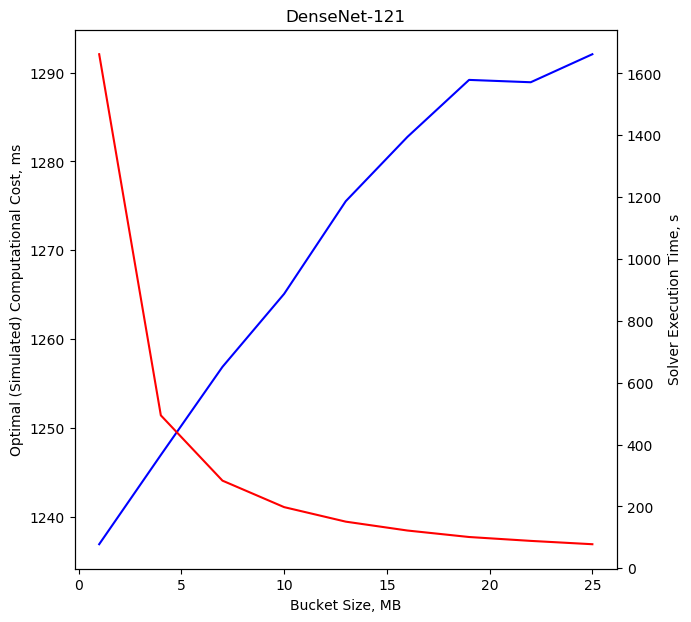
\includegraphics[width=0.6\linewidth]{optimal_cost_and_solver_exec_time_vs_bucket_size.png}
    \caption{Optimal cost (blue) and solver execution time (red) against bucket size, for DenseNet-121.}
    \label{fig:4-bucket-size}
\end{figure}

At the left side of the graph, with a bucket size of just under 1MB, we see that the solver takes 26 minutes to complete.
I think this is acceptable for networks like this that take a large number of hours to train.
As we increase the bucket size, the execution time drops drastically, before starting to level out.
This will be due to the large sequence size starting to dominate the time complexity instead of the memory budget.
At a reasonable bucket size of 5MB, the execution time has dropped 75\% to ~7 minutes.
Thus, this increased bucket size is already more than practical, and the corresponding increase in computational cost is little over 1\%.
I think it is therefore reasonable to conclude that the large memory budget and resulting bucketing has not greatly inhibited the solver's practicality.

During experimentation, it is quite feasible that researchers may want to run a large model for a short period of time.
In that case, even 7 minutes of waiting for the solver could be annoying.
Thus, I explored bucketing further.
We can see from the graph that, for the very large bucket size of 25MB, the execution time has dropped all the way to under a minute, which should be satisfactory in such a use case.
The optimal computational cost has risen from the origin 1235ms to 1900ms, an overhead of 53\%.
This is still reasonable, especially considering the stated use case was for models that will only be run for a short period of time.
Clearly, enabling checkpointing will by far easier, cheaper and quicker for the researcher than implementing distribution to overcome the memory requirement.
